\documentclass[a4paper,12pt,twoside]{article}
\usepackage{rhreport}

\title{Aerial Riparian Solid Waste Mapping}
\author{OpenMap Development Tanzania}


\date{July 2019}

\begin{document}


\maketitle

This report was prepared by Glory Emanuel, Bornlove Ntikha, Iddy Chazua, Dorica Mugusi, Tonny John, Immaculate Mwanja\footnote{test}, Aaron Eubank, Hawa Adinani, Innocent Maholi, Ivan Gayton, William Evans


\newpage
\tableofcontents

\newpage
\section{Executive Summary}
\begin{multicols}{3}

\lipsum[0-3]

\end{multicols}

\section{Introduction}

\lipsum[0-4]
  
Drone flights enable studying any aggregations of waste/informal dumps that are on the banks of the waterways within fifty metres of its bank on either side.Such data is presented as three-dimensional imagery of waste aggregations, further assisting the study team to estimate rough waste volumes.

Drone flights consistently track and record spatial data relating to their own trips and correspond the GIS data with a set of other socio-political and economic indicators, to ease further analysis. This includes:   

\begin{itemize}
    \item The corresponding political division i.e. subward, ward and municipal boundaries—drone flight spatial data overlaid existing socio-political spatial data indicating, via simple desktop analysis, the political constituency that governs each spatial area the drone covers. This allows users to correspond with an informal/illegal dump with the relevant political office that governs the area.
    \item The corresponding density of the geography they are flown over i.e. buildings per sq km/population per sq km via census data. 
\end{itemize}



OMDTZ  combined drone flights and the existing spatial data to conduct a rapid desktop analysis of planned residential and commercial zoning and transport economics as they relate to solid waste management services.

Specifically, spatial analysis allowed the team to quickly present:
\begin{itemize}
    \item Any building or point on a map within the political boundaries of Dar es Salaam that are defined as planned or unplanned.
    \item The complexity of transport from any building in Dar es Salaam to Pugu Kinyamwezi dump site---accounting for two-axle vehicle access, road surface and type, distance and time. 
\end{itemize}
    
Datasets provided audiences with vital data on the inequality of solid waste management infrastructure by geography, as well as providing service providers and government with valuable data on what types of transport modes can be employed to service residents and businesses in planned and unplanned geographies of the city.  

Thereafter, OpenDataKit (ODK) Collect,Kobo Toolbox & QGIS trainings were provided to Nipe Fagio staff. OMDTZ provided an in-depth training on how to upload, analyze and present visual data relating to waste hotpots, informal dumps and cleaning activities.


\newpage
\section{Objectives}

    The broad purpose of this work is to provide Nipe Fagio, I4ID and other partners with high-quality and interactive spatial data to better understand solid waste management and service quality across all five municipalities of Dar es Salaam. The main focus of the activities will be along all of the city’s key five rivers which are Mpiji, Tegeta, Mzinga, Kizinga and Msimbazi rivers.

        \begin{figure}%[H] % uncomment "[H]" to force the image to the middle of the page
            \centering
            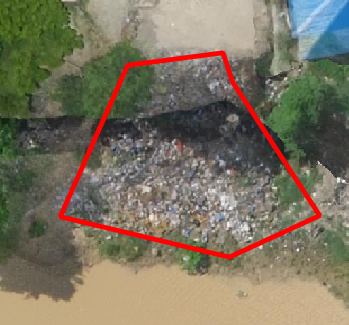
\includegraphics[width=0.8\textwidth]{images/image17.png}
            \caption{Screenshot showing missions plans of river mapping}
        \end{figure}

\section{Stakeholders}

\subsection{Implementing Partners}

    \begin{itemize}
        \item \textbf{OpenMap Development Tanzania (OMDTZ)} %\textbf{} bolds the items
    
        OpenMap Development Tanzania (OMDTZ) is a local registered NGO based in Dar es Salaam and operating across Tanzania. Since its establishment, OMDTZ has promoted a number of community mapping projects, generated map awareness, actively pledged open data sets and continued to build a network of enthusiastic mappers in Tanzania.
    
        \item \textbf{UhuruLabs}
    
        UhuruLabs aims to leverage technology and innovation for the development and benefit of Africa and its people. UhuruLabs believes in a world where Africa is an equal and fair beneficiary of its own resources and can take full advantage of technological advancements being made across the world. Projects range from the developing of a multi-rotor drone specifically for use in African agriculture to developing the idea open source toolchain for processing high resolution drone imagery. 
    
        UhuruLabs provided the drones that were used to take the 5cm resolution aerial imagery for mapping four out of five major rivers━Mpiji, Tegeta, Kizinga and Mzinga━in Dar es Salaam city.
    
    \end{itemize}

\subsection{Beneficiaries}

    \begin{itemize}
        \item \textbf{Nipe Fagio}
    
        Nipe Fagio, “Give Me the Broom” in Swahili, is a civil society organization founded in 2013. It aims to empower individuals, especially the youth, the civil society, the private sector and government to build lasting change towards turning Tanzania into a clean and sustainable country, conscious through education of its role on waste management and reduction of pollution (air, water, soil).
    
        Nipe Fagio staff were trained by OMDTZ on the use of OpenStreetMap (OSM) local tools for data collection and to use Geographic Information Systems (GIS) to address the issue of waste in the city under their Zero Waste project. QGIS software was executed after the training.

        \item \textbf{Institutions for Inclusive Development (I4ID)}
    
        I4ID are Tanzanian institutions working to the systems that drive poverty and exclusion. They bring actors together, to design and implement innovative solutions that have the potential for large scale impact.
    
    \end{itemize}

\subsection{Funders}

    \begin{itemize}
        \item \textbf{Palladium}
    
        \lipsum[0-1]
    
    \end{itemize}   

\section{Activity 1: UAV Data Collection}

\subsection{Drone Use}

    Drone is a popular name of Unmanned Aerial Vehicles (UAV) that uses Unmanned Aerial System (UAS) for the different purposes according to the manufacturer Operation manual or User preference. 

Several drone flights were to be  conducted along five major rivers of Dar es Salaam including  Msimbazi, Mpiji, Tegeta, Kizinga and Mzinga rivers, spanning 60 linear kilometers of waterways of Dar es Salaam’s critical water arteries. Msimbazi river was not mapped since it  was  already mapped by World bank. The drone flights provided a digital photographic mark-up of the current status of Dar es Salaam’s waterways. 

Drone flights for data collection were conducted within 44 calendar days from 5th April to 18th May 2019, contingent  to the Tanzania Civil Aviation Authority (TCAA) and Ministry of Defence permissions and suitable weather. All technical personnel and equipment required for this assignment are present in Dar es Salaam (site location). 

\subsection{Tools}

    During data collection, the following tools were used in site activities:
    \begin{itemize}
  
        \item Spare wings for specific drones (\href{https://www.sensefly.com/solution/ag-360-agricultural-drone/ebee-plus-4/}{ebee plus}\footnote{\url{https://www.sensefly.com/solution/ag-360-agricultural-drone/ebee-plus-4/}})
        \item Spare propellers and rubber to hold the propeller in place
        Umbrella for sunshade used to protect our facilities from rain and sun but also ourselves.
        \item Lithium Polymer (Lipo) batteries and it is bag; enough batteries were packed in the lipo battery bag to help mitigate damage and fire risk to the surrounding objects. Lipo battery bag can save resulting from batteries explosion or fire. Therefore the batteries were packed in the lipo battery bag to ensure safety. 
        \item Radio tracker; this was used to keep track of the drone once it is activated in the drone. This means that you will keep track of the drone, provided that it has this device with it and on, on board you will have Radio Transmitter and on the ground you will have radio receiver in which the radio transmitter will emit radio signals of dedicated frequency in which with your receiver you have to squawk the frequency that will match with that coming from the transmitter on board thus will produce the sound to indicate the matching frequency. How to locate the Drone that has radio Transmitter on it will be simply by using receiver to point on different direction fetching for the where the radio is coming from, once you get the strong signal, you will bet the clean beeping sound from the noise beeping sound, then you will have to move towards the direction where the clean sound is made.
        \item UHU Glue for Polystyrene minor repair
        \item MicroSD cards for swapping
        \item Reflector vest
    
    \end{itemize}

\subsection{Drone Processes}

    \begin{multicols}{2}
    eBee drones (version Plus and X) were used during the river mapping project to track and record spatial data related to their own trips and corresponding GIS data with a set of other socio-political and economic indicators to ease further analysis. Drone imagery is the output of Unmanned Aerial Vehicle (UAV) carrying a camera to conduct imaging mission. The image is then GeoTagged with Drone Log data that is stitched together to get the output according to the pilot’s desire (Orthomosaic). After the processes explained above, the images were compressed for further use on light processing machines like mobile phones for mapping exercises of trash point location identification.
    \end{multicols}
    
\section{Activity 2: Remote Data Collection}

\section{Activity 3: Training of Nipe Fagio Personnel}

\subsection{Executive Summary}

    \begin{multicols}{2}
    \lipsum[0-5]
    \end{multicols}

\subsection{Objectives}

    \begin{multicols}{2}
    \lipsum[0-5]
    \end{multicols}

\subsection{OpenDataKit (ODK) Collect Training}

    \begin{multicols}{2}
    \lipsum[0-5]
    \end{multicols}

\subsection{QGIS Training}

    \begin{multicols}{2}
    \lipsum[0-5]
    \end{multicols}

\subsection{Creation of Kobo Toolbox  server for data aggregation}

    \begin{multicols}{2}
    \lipsum[0-5]
    \end{multicols}
	
\subsection{Data Collection Tools}

    \begin{multicols}{2}
    \lipsum[0-5]
    \end{multicols}

\subsection{Map Literacy}

    \begin{multicols}{2}
    \lipsum[0-5]
    \end{multicols}

\subsection{Preparation of Building Clustering and Non-clustering Randomization Manuals}

    \begin{multicols}{2}
    \lipsum[0-5]
    \end{multicols}

\subsection{Waste Management Pilot in Mapped Areas With Nipe Fagio}

    \begin{multicols}{2}
    \lipsum[0-5]
    \end{multicols}

\subsection{Questionnaire}

    \begin{multicols}{2}
    \lipsum[0-5]
    \end{multicols}

\subsection{Data Cleaning using OpenRefine}

    \begin{multicols}{2}
    \lipsum[0-5]
    \end{multicols}

\subsection{Preparation of Interactive Web Map}

    \begin{multicols}{2}
    \lipsum[0-5]
    \end{multicols}

\section{Activity 4: Routing}

\section{Conclusion}

    \begin{multicols}{2}
    \lipsum[0-5]
    \end{multicols}

\subsection{Achievements}

    \begin{multicols}{2}
    \lipsum[0-5]
    \end{multicols}

\subsection{Challenges}

    \begin{multicols}{2}
    \lipsum[0-5]
    \end{multicols}

\subsection{Lessons Learned}

    \begin{multicols}{2}
    \lipsum[0-5]
    \end{multicols}
    
\subsection{Recommendations}

    \begin{multicols}{2}
    \lipsum[0-5]
    \end{multicols}

\section{Acknowledgements}

    \begin{multicols}{2}
    \lipsum[0-5]
    \end{multicols}

\section{References}

    \begin{multicols}{2}
    \lipsum[0-5]
    \end{multicols}

\end{document}

